% Created 2017-05-13 Sat 18:47
% Intended LaTeX compiler: pdflatex
\documentclass[presentation]{beamer}
\usepackage[utf8]{inputenc}
\usepackage[T1]{fontenc}
\usepackage{graphicx}
\usepackage{grffile}
\usepackage{longtable}
\usepackage{wrapfig}
\usepackage{rotating}
\usepackage[normalem]{ulem}
\usepackage{amsmath}
\usepackage{textcomp}
\usepackage{amssymb}
\usepackage{capt-of}
\usepackage{hyperref}
\usetheme{default}
\author{bachir el khadir}
\date{\today}
\title{}
\begin{document}

\begin{frame}{Outline}
\tableofcontents
\end{frame}

\scalebox{.5}\{
\begin{figure}
\centering
\hspace*{-.75in}
   \begin{tikzpicture}[scale=0.5\textwidth]\begin{scope}[every node/.style={circle,thick,draw}]
\node (1) at (5.12,0.00) {1};
\node (2) at (0.0,3.31) {2};
\node (3) at (7.25,3.52) {3};
\node (4) at (9.85,0.23) {4};
\node (5) at (3.92,6.79) {5};
\node (6) at (10, 7) {6};
\node (7) at (15,8.83) {7};
\node (8) at (6.10,10.44) {8};
\node (9) at (6.20,15.88) {9};
   \end{scope}\begin{scope}[>={Stealth[black]},
   every node/.style={fill=white,circle},
   every edge/.style={draw=red,very thick}]
   \path [->] (1) edge[bend left=20] node {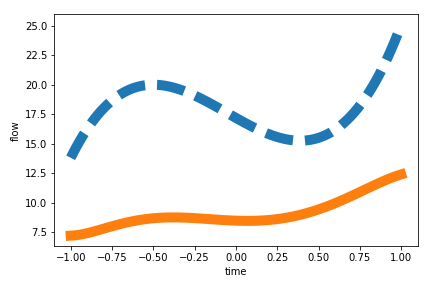
\includegraphics[width=0.05\textwidth]{includes/edges_flow/flow1-2.png}} (2);
\path [->] (1) edge node {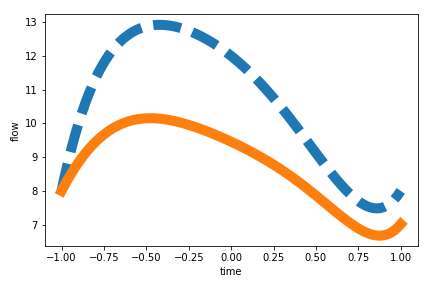
\includegraphics[width=0.05\textwidth]{includes/edges_flow/flow1-3.png}} (3);
\path [->] (1) edge node {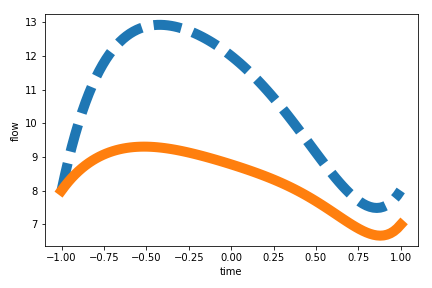
\includegraphics[width=0.05\textwidth]{includes/edges_flow/flow1-4.png}} (4);
\path [->] (1) edge node {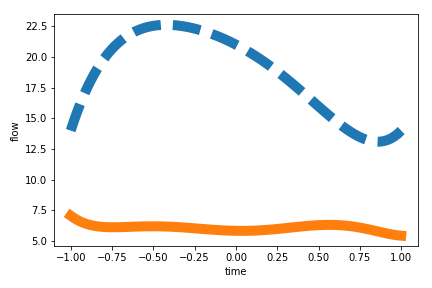
\includegraphics[width=0.05\textwidth]{includes/edges_flow/flow1-5.png}} (5);
\path [->] (2) edge node {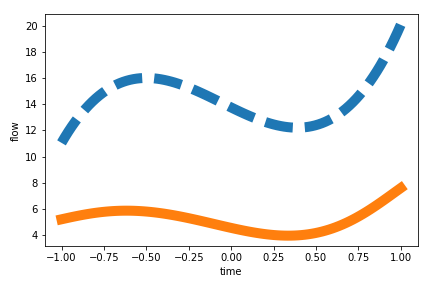
\includegraphics[width=0.05\textwidth]{includes/edges_flow/flow2-5.png}} (5);
\path [->] (2) edge[bend left=40] node {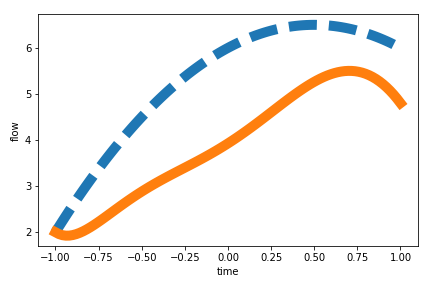
\includegraphics[width=0.05\textwidth]{includes/edges_flow/flow2-9.png}} (9);
\path [->] (3) edge node {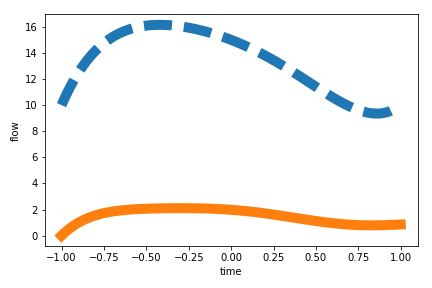
\includegraphics[width=0.05\textwidth]{includes/edges_flow/flow3-5.png}} (5);
\path [->] (3) edge node {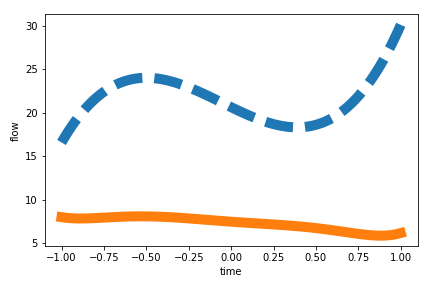
\includegraphics[width=0.05\textwidth]{includes/edges_flow/flow3-6.png}} (6);
\path [->] (4) edge node {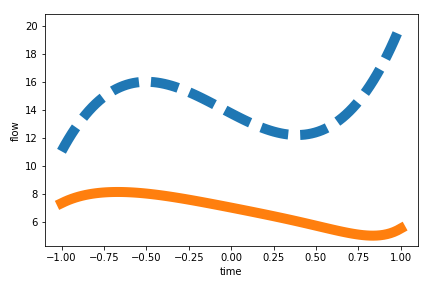
\includegraphics[width=0.05\textwidth]{includes/edges_flow/flow4-6.png}} (6);
\path [->] (4) edge[bend right=20] node {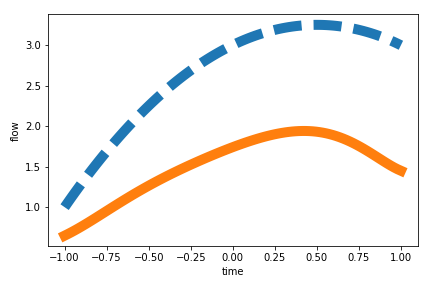
\includegraphics[width=0.05\textwidth]{includes/edges_flow/flow4-7.png}} (7);
\path [->] (5) edge node {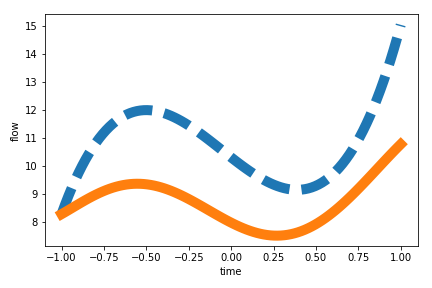
\includegraphics[width=0.05\textwidth]{includes/edges_flow/flow5-8.png}} (8);
\path [->] (5) edge[bend left=20] node {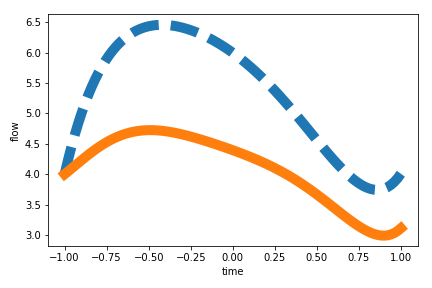
\includegraphics[width=0.05\textwidth]{includes/edges_flow/flow5-9.png}} (9);
\path [->] (6) edge node {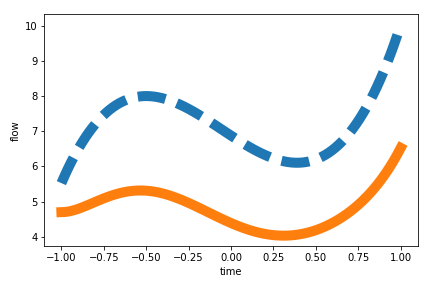
\includegraphics[width=0.05\textwidth]{includes/edges_flow/flow6-7.png}} (7);
\path [->] (6) edge node {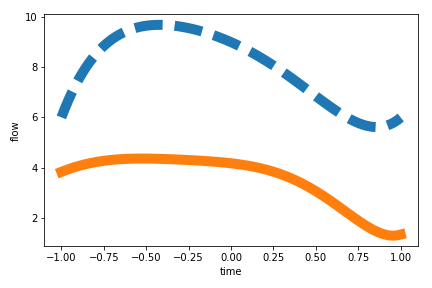
\includegraphics[width=0.05\textwidth]{includes/edges_flow/flow6-8.png}} (8);
\path [->] (6) edge[bend right=20] node {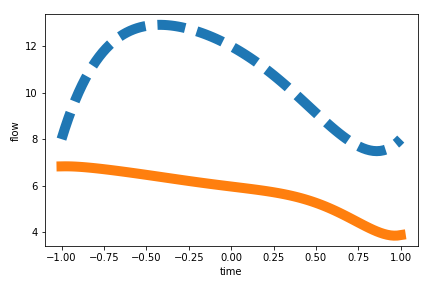
\includegraphics[width=0.05\textwidth]{includes/edges_flow/flow6-9.png}} (9);
\path [->] (7) edge[bend right=40] node {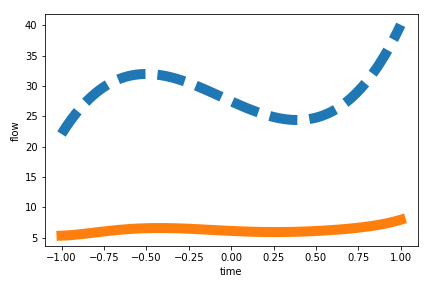
\includegraphics[width=0.05\textwidth]{includes/edges_flow/flow7-9.png}} (9);
\path [->] (8) edge node {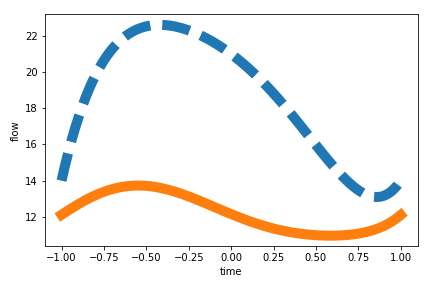
\includegraphics[width=0.05\textwidth]{includes/edges_flow/flow8-9.png}} (9);
   \end{scope}\end{tikzpicture}
\caption{MAXFLOW}
\end{figure}
\}
\end{document}